\documentclass[14pt]{beamer}
%\usetheme[compress]{Singapore} % Guia no alto, nada mais, degrade azul
\usetheme{Frankfurt} % Guia no alto, nada mais

\usepackage{multirow}

\title{Economically-Efficient\\Data Stream Analysis}
\author{\small{Roberto Oliveira Jr.\\Advisor: Adriano Veloso \\Co-advisor: Wagner Meira Jr.}}
\institute{Computer Science Dept - UFMG - Brazil}
\date{}

\begin{document}

\begin{frame}
\titlepage
\end{frame}

\section{Data Stream Analysis}

\begin{frame}\frametitle{Data Stream}

\begin{itemize}
\item Definition
\begin{itemize}
\item Fast and possible unbounded sequence of data that arrives at time-varying.
\end{itemize}
\item Motivation
\begin{itemize}
%\item Twitter, and other text-based channels, produce torrents of opinionated content.
\item It allows us to process huge volumes of data.
%It allows us to track products, brands and people to determine whether they are viewed positively or negatively.
\end{itemize}
\end{itemize}
\begin{itemize}
\item Problem
\begin{itemize}
\item Automatically extraction of relevant patterns and relations from data that is continuously created.
%Content is created almost at the same time the event is happening in the real world.
\begin{itemize}
\item Keep track of data streams is useful for systems monitoring, online social network advertising, etc.
%Keeping track of \alert{sentiment streams} is useful for advertising.
\end{itemize}
\end{itemize}
\end{itemize}

\end{frame}

%\begin{frame}\frametitle{Sentiment Streams and Outbreaks}
%
%{\underline{Dengue Fever}}
%
%\begin{figure}
%\centering
%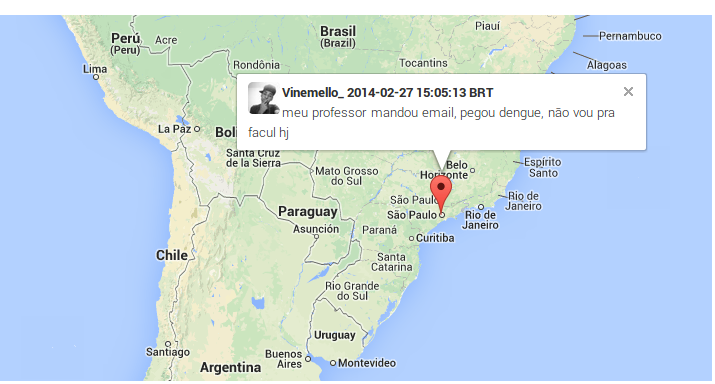
\includegraphics[height=2.30in]{ow2}
%\end{figure}
%
%\end{frame}

\begin{frame}\frametitle{Social Networks Streams and Advertising}

{\underline{Superbowl 2013}}

\begin{figure}
\centering
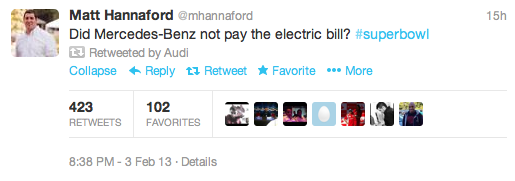
\includegraphics[height=1.30in]{mercedez}
\end{figure}
\vspace{-0.1in}
\begin{figure}
\centering

\includegraphics[height=1.10in]{audi}
\end{figure}

\end{frame}

% \begin{frame}\frametitle{Sentiment Streams and Advertising}

% and last year ... Brazil 1 $\times$ Germany 7

% \begin{figure}
% \centering
% 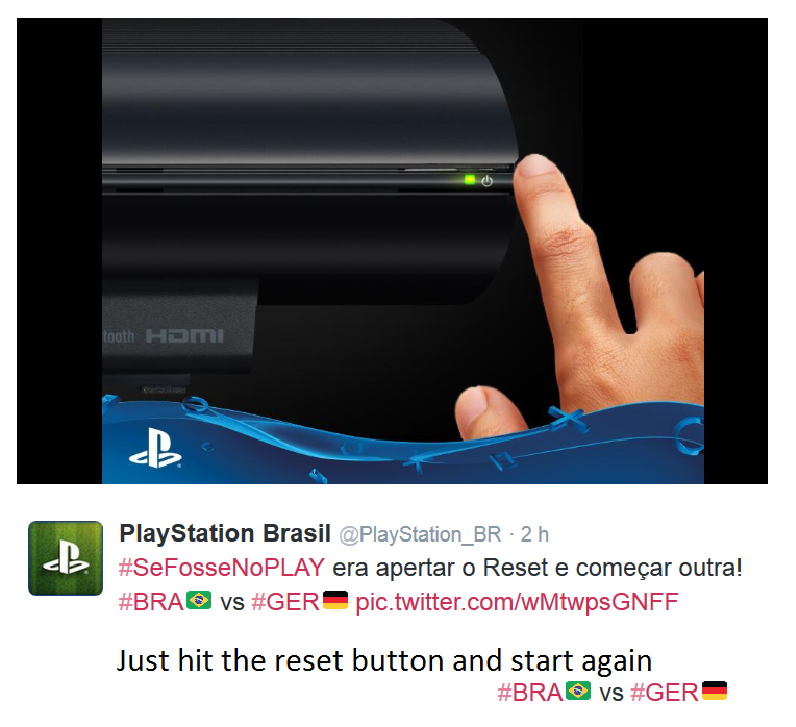
\includegraphics[height=2.50in]{playstation}
% \end{figure}

% \end{frame}

%\begin{frame}\frametitle{Sentiment Streams and Advertising}
%
%and yesterday ... Brazil 1 $\times$ Germany 7
%
%\begin{figure}
%\centering
%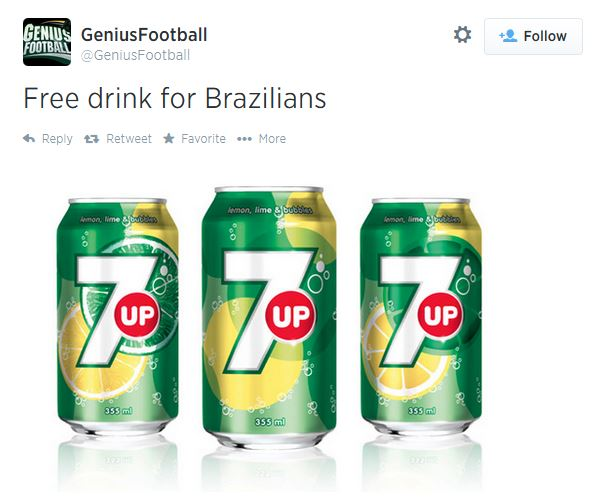
\includegraphics[height=2.50in]{sevenup}
%\end{figure}
%
%\end{frame}

\begin{frame}\frametitle{Classifying Data Streams}

\begin{itemize}
\item Classifiers are applied to distinguish between pre-defined labels.
%Classifiers may be used to distinguish sentiments in the text.
\end{itemize}

\vspace{-0.2in}
\begin{figure}
\centering
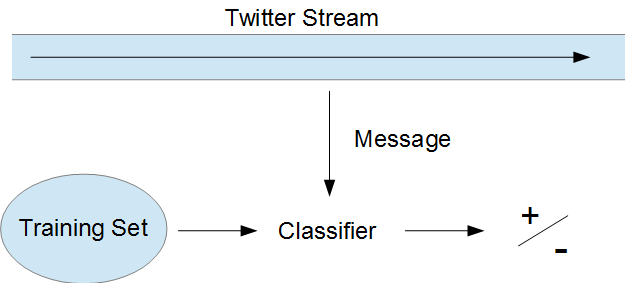
\includegraphics[height=1.30in]{stream1}
\end{figure}
\vspace{-0.2in}
\pause
\begin{itemize}
\item \alert{Data characteristics may change with time}.
\end{itemize}
\end{frame}

\begin{frame}\frametitle{Concept Drifts Types}
\begin{itemize}
\item Most common types of Concept Drifts:
\end{itemize}

\vspace{0.1in}
\begin{figure}
\centering
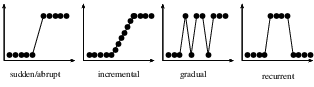
\includegraphics[scale=1]{concept_drift}
\end{figure}
%\vspace{-0.2in}
\pause
\begin{itemize}
\item Data streams contains combination of such concept drifts types.
\end{itemize}
\end{frame}


\begin{frame}\frametitle{Sports (WC 2010)}

\vspace{-0.1in}
\begin{figure}
\centering
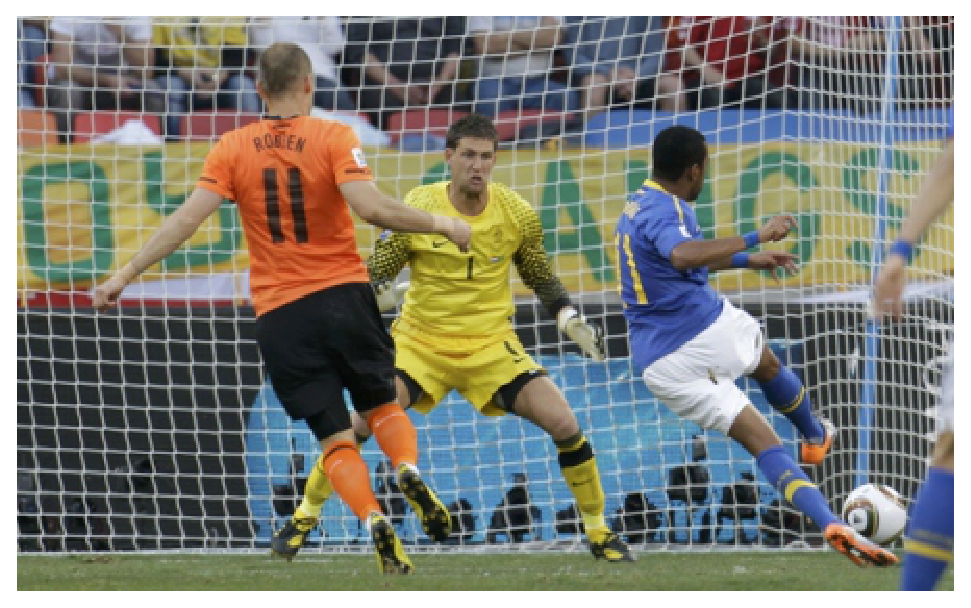
\includegraphics[height=1.00in]{golrobinho.eps}
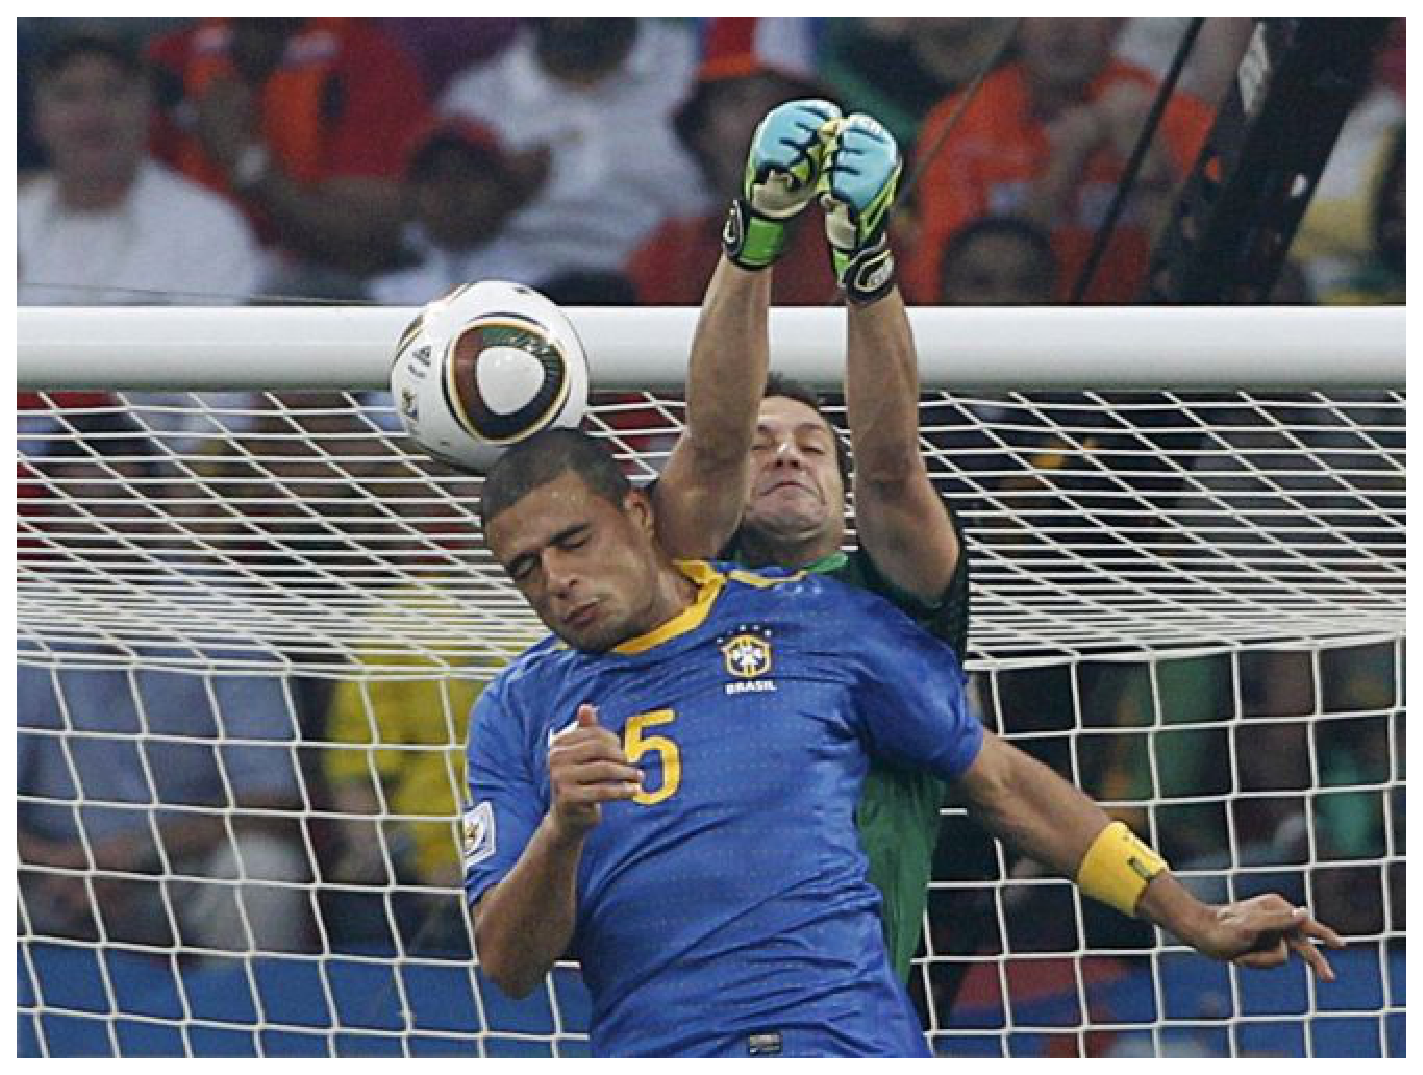
\includegraphics[height=1.00in]{contra.eps}
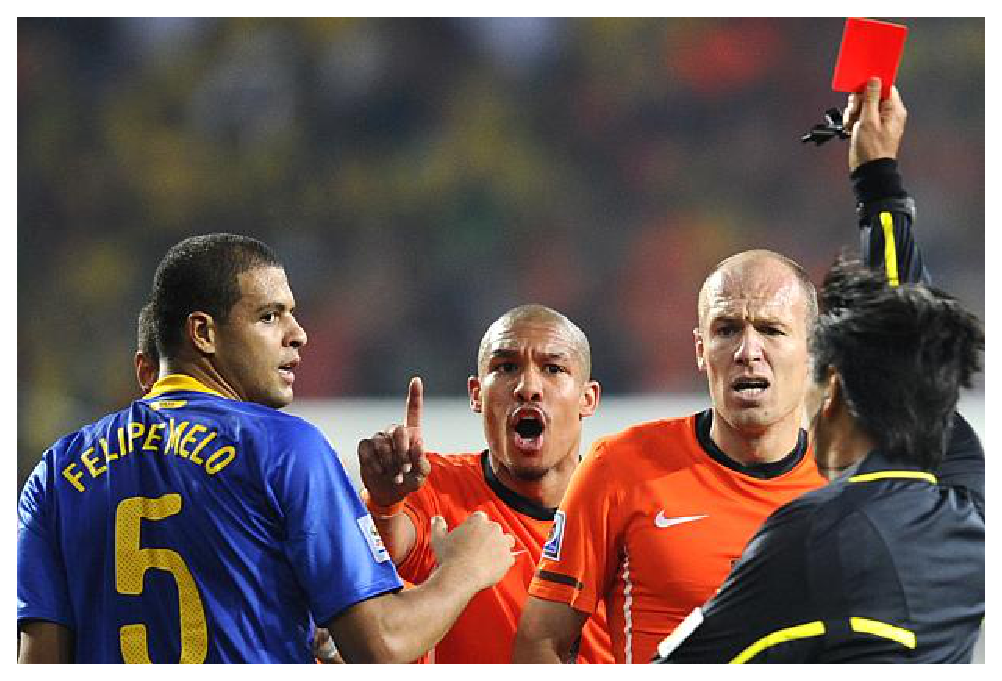
\includegraphics[height=1.00in]{vermelho.eps}
\end{figure}

\vspace{-0.15in}
\begin{figure}
\centering
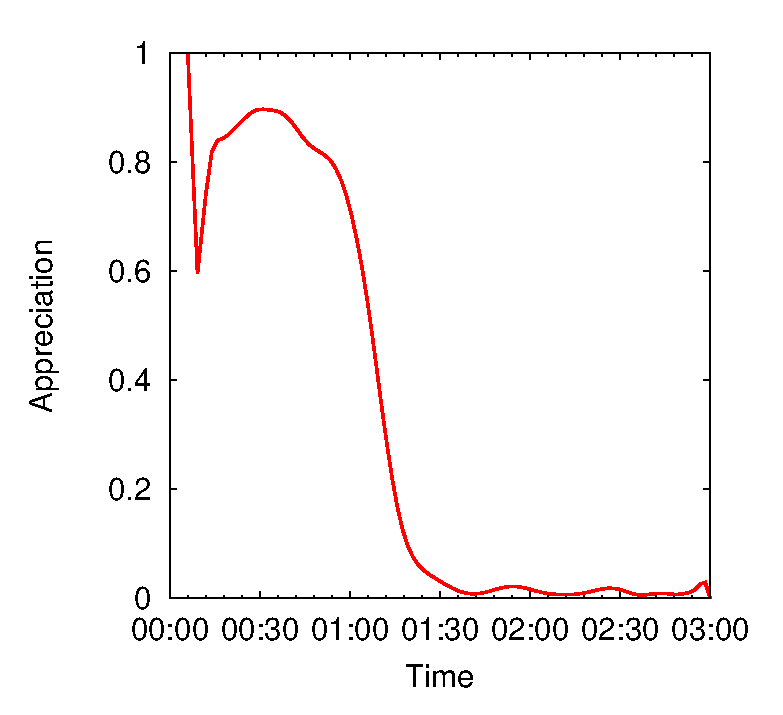
\includegraphics[width=2.35in,height=1.75in]{felipemeloPositividade.eps}
\end{figure}

\end{frame}

\begin{frame}\frametitle{Elections (Brazil 2010)}

\vspace{-0.1in}
\begin{figure}
\centering
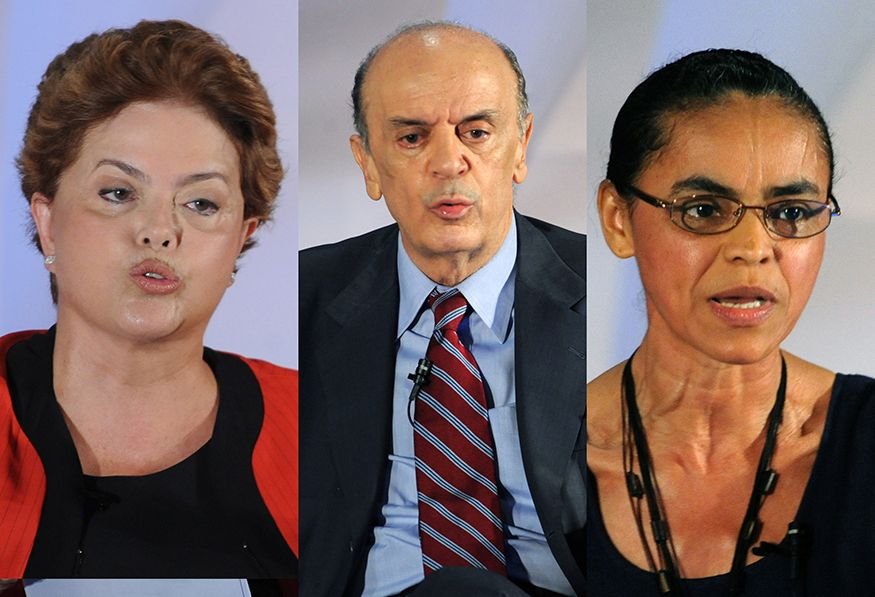
\includegraphics[height=0.95in]{dilma1}
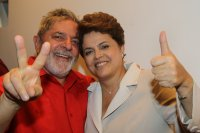
\includegraphics[height=0.95in]{lula}
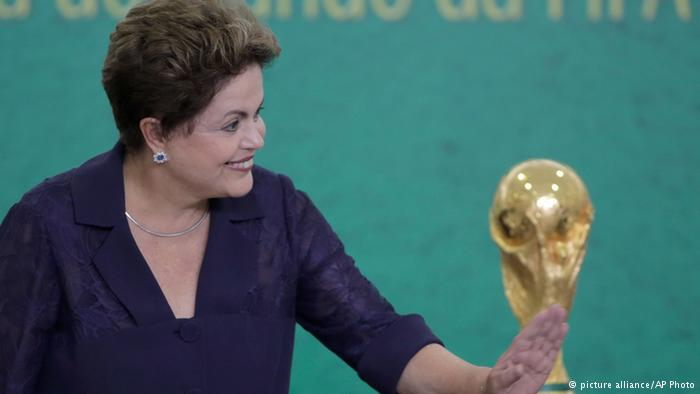
\includegraphics[height=0.95in]{copa}
\end{figure}

\vspace{-0.15in}
\begin{figure}
\centering
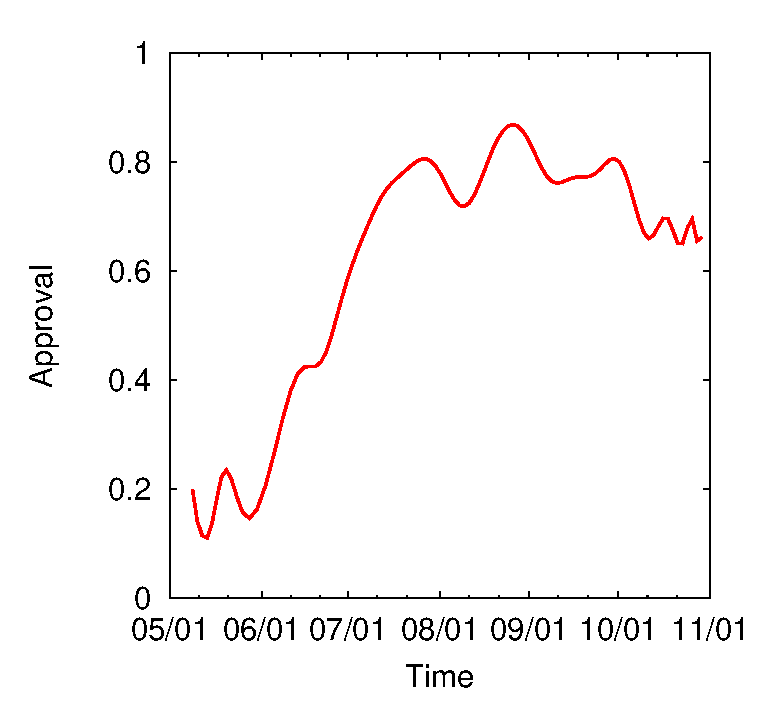
\includegraphics[width=2.35in,height=1.75in]{dilmaPositividade.eps}
\end{figure}

\end{frame}

\begin{frame}\frametitle{Classifying Data Streams}

\begin{itemize}
\item Effective classification requires:
\begin{itemize}
\item Updating the classification model as the stream evolves.
\begin{itemize}
\item Account for limited resoucres: memory, time and learning requirements.
\end{itemize}
\end{itemize}
\end{itemize}

\vspace{-0.2in}
\begin{figure}
\centering
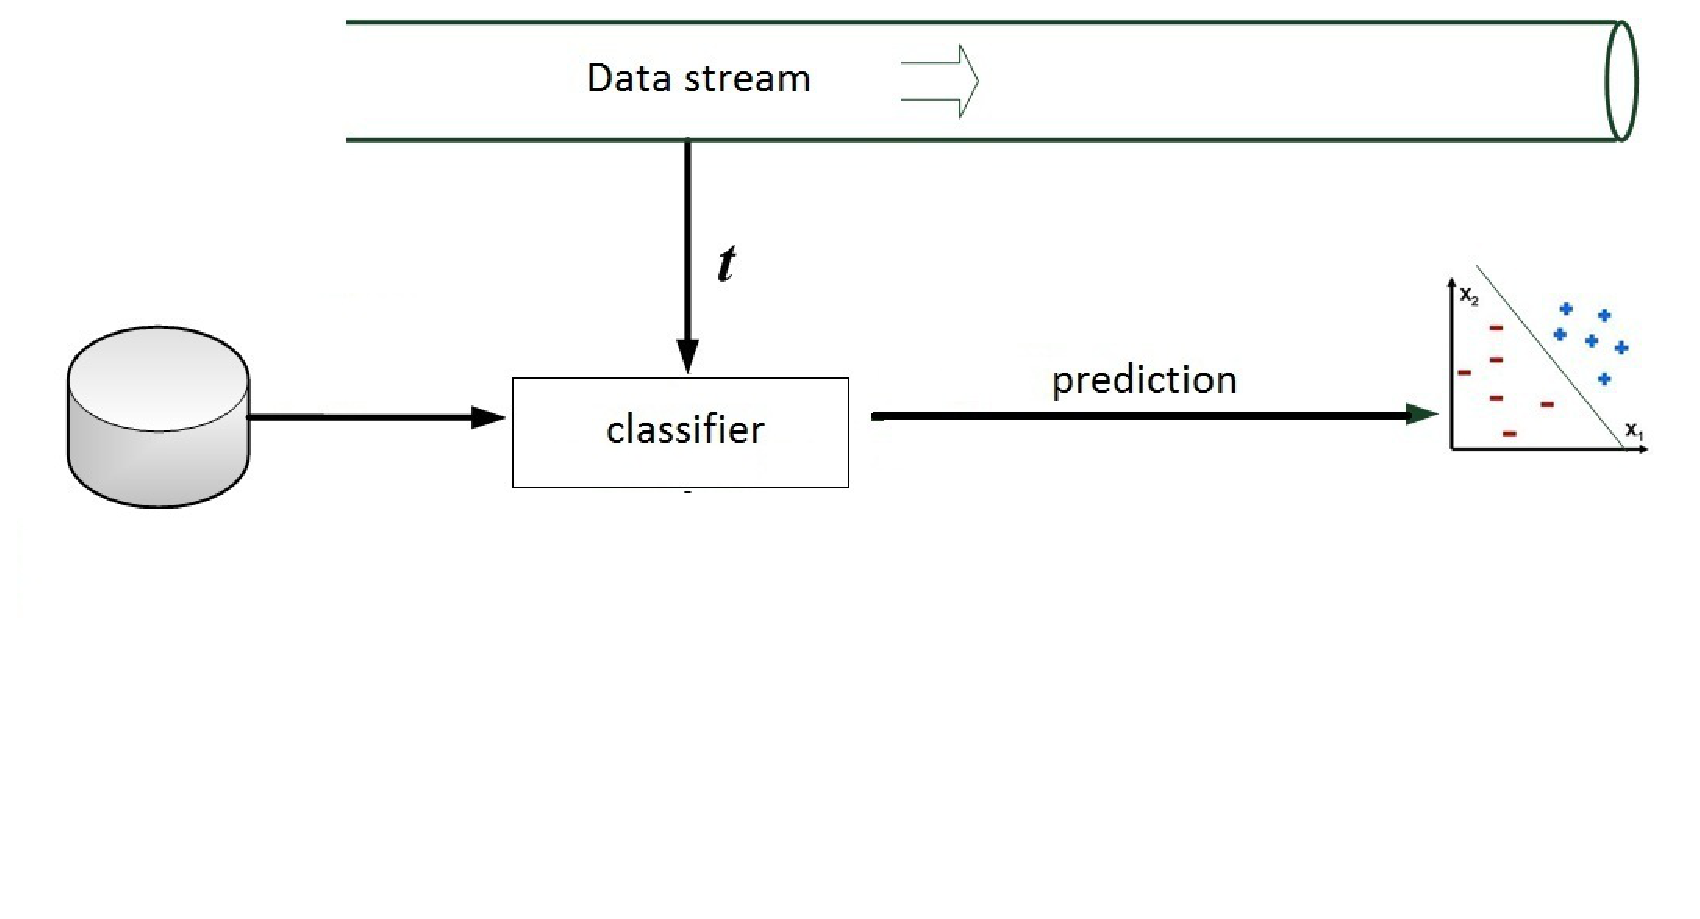
\includegraphics[height=1.60in]{stream2}
\end{figure}
\end{frame}


\begin{frame}\frametitle{Research Question}

\begin{itemize}
\item How to deal with concept drifts?
\end{itemize}

\end{frame}


% \begin{frame}\frametitle{Research Questions}

% \begin{enumerate}
% \item Resources:
% \begin{itemize}
% \item \alert{How to build classification models fast?}
% \end{itemize}

% \item Accuracy:
% \begin{itemize}
% \item How to deal with concept drifts?
% \end{itemize}

% \item Effort:
% \begin{itemize}
% \item How to reduce labeling effort?
% \end{itemize}

% \end{enumerate}

% \end{frame}

% \section{Classification Model}
% \begin{frame}
% \frametitle{Classification Model}%Lightweight Classifiers}

% \begin{itemize}
% \item Our classification model $\mathcal{R}$ is composed of rules $\{X\to c_i\}$.
% \begin{itemize}
% \item $X$ is any combination of features in the target instance.
% \item $c_i$ is a label.
% \end{itemize}
% \end{itemize}

% \end{frame}


% \begin{frame}\frametitle{Label Scoring}

% \begin{itemize}
% \item Given a target instance $t_n$:
% \begin{enumerate}
% \item Build a classification model $\mathcal{R}(t_n)$ composed of rules $\{X\to c_i\}$ for which $X\subseteq t_n$.
% \item The label score is given by the linear combination of the rules.
% \end{enumerate}
% \end{itemize}

% \pause

% {\small{``It works well, my sister loves it, but unfortunatelly it broke.''}}

% \begin{itemize}
% \item $\{$broke$\}\to$ negative (0.77)
% \item $\{$work, well$\}\to$ positive (0.85)
% \item $\{$love, it$\}\to$ positive (0.91)
% \end{itemize}
% \end{frame}


% \section{Labeling Effort}

% \begin{frame}\frametitle{Research Questions}

% \begin{enumerate}
% \item Resources:
% \begin{itemize}
% \item \alert{How to build classification models fast?}
% \end{itemize}

% \item Accuracy:
% \begin{itemize}
% \item How to deal with concept drifts?
% \end{itemize}

% \item Effort:
% \begin{itemize}
% \item \alert{How to reduce labeling effort?}
% \end{itemize}

% \end{enumerate}

% \end{frame}

\section{Drifts}

% \begin{frame}\frametitle{Research Questions}

% \begin{enumerate}
% \item Resources:
% \begin{itemize}
% \item How to build classification models fast?
% \end{itemize}

% \item Accuracy:
% \begin{itemize}
% \item \alert{How to deal with concept drifts?}
% \end{itemize}

% \item Effort:
% \begin{itemize}
% \item How to reduce labeling effort?
% \end{itemize}

% \end{enumerate}

% \end{frame}


\begin{frame}\frametitle{Dealing with Drifts}

\begin{itemize}
\item Two properties are necessary in order to produce classifiers that are robust to drifts:
\begin{itemize}
\item Adaptiveness:
\begin{itemize}
\item The ability to adapt itself to drifts.
\end{itemize}
\item Memorability:
\begin{itemize}
\item The ability to recover itself from drifts.
\end{itemize}
\end{itemize}
\end{itemize}

\begin{figure}
\centering
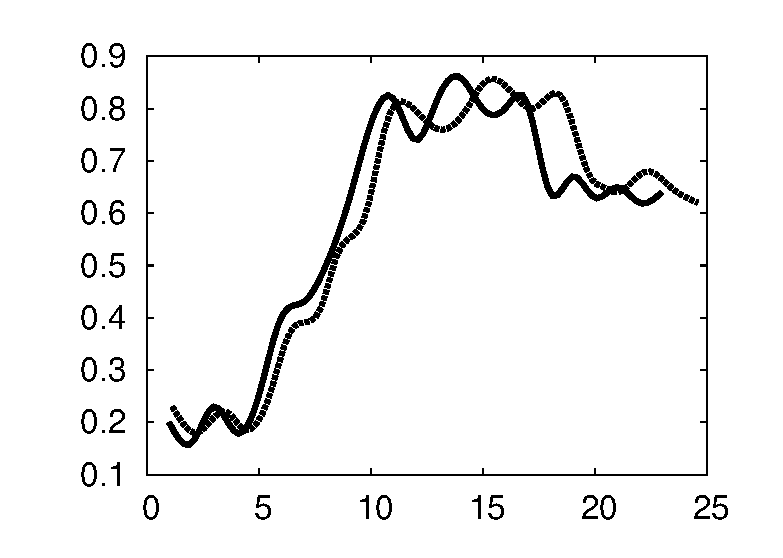
\includegraphics[height=1.30in]{drift3}
\end{figure}
\end{frame}

\begin{frame}\frametitle{Dealing with Drifts}

\begin{itemize}
\item Two properties are necessary in order to produce classifiers that are robust to drifts:
\begin{itemize}
\item Adaptiveness:
\begin{itemize}
\item The ability to adapt itself to drifts.
\item The training-set must contain fresh messages.
\end{itemize}
\item Memorability:
\begin{itemize}
\item The ability to recover itself from drifts.
\item The training-set must contain pre-drift messages.
\end{itemize}
\end{itemize}
\item Improving both properties simultaneously may lead to a conflict-objective problem.
\begin{itemize}
\item Improve adaptiveness may hurt memorability, and vice-versa.
\end{itemize}
\end{itemize}

\end{frame}


\begin{frame}\frametitle{Pareto Efficiency}

Example: hotels in Petr\'{o}polist.

\begin{figure}
\centering
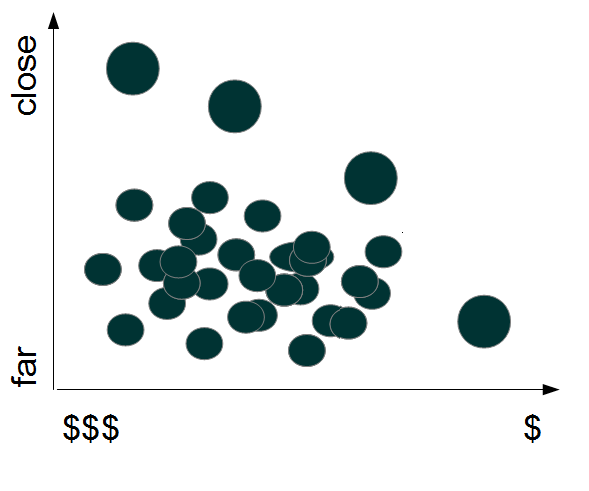
\includegraphics[height=1.60in]{hotel1}
\end{figure}

\end{frame}

\begin{frame}\frametitle{Pareto Efficiency}

Pareto frontier.

\begin{figure}
\centering
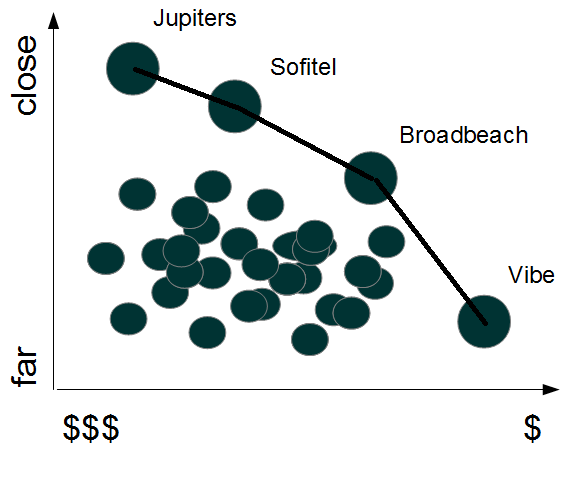
\includegraphics[height=1.60in]{hotel2}
\end{figure}

\end{frame}

\begin{frame}\frametitle{Compensation $-$ Kaldor-Hicks Principle}

Region of compensation.

\begin{figure}
\centering
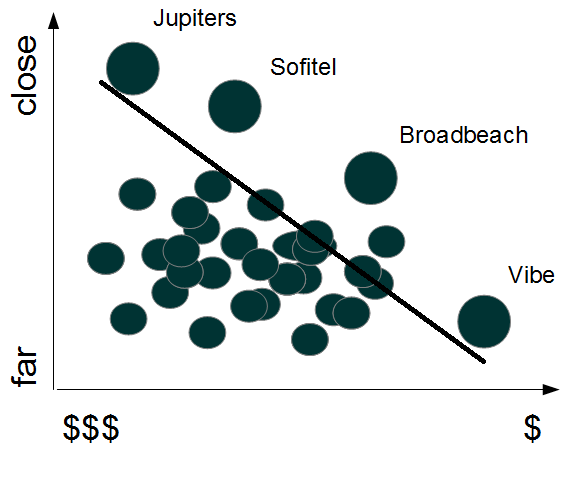
\includegraphics[height=1.60in]{hotel3}
\end{figure}

\end{frame}



\begin{frame}\frametitle{Utility Measures}

\begin{itemize}
\item Distance in space:
\begin{itemize}
\item How similar message $t_j$ is to the newest message $t_n$.
\item $U_s(t_j)=\frac{|\mathcal{R}(t_n) \cap \mathcal{R}(t_j)|}{|\mathcal{R}(t_n)|}$
\end{itemize}
\item Distance in time:
\begin{itemize}
\item How fresh is the message.
\item $U_t(t_j)=\frac{\gamma(t_j)}{\gamma(t_n)}$.
\begin{itemize}
\item $\gamma(t_j)$ returns the time in which message $t_j$ arrived.
\end{itemize}
\end{itemize}
\item Random permutation of messages:
\begin{itemize}
\item $U_r(t_j)=\frac{\alpha(t_j)}{|\mathcal{D}_n|}$
\begin{itemize}
\item $\alpha(t_j)$ returns the position of $t_j$ in the shuffle.
\item $\mathcal{D}_n$ is the training set at time step $n$.
\end{itemize}
\end{itemize}
\end{itemize}

\end{frame}

\begin{frame}\frametitle{Utility Measures}

\begin{enumerate}
\item At each time step $n$:
\begin{enumerate}
\item Place candidate messages in the utility space.
\item Select messages in the Pareto frontier.
\end{enumerate}
\end{enumerate}

\vspace{-0.1in}
\begin{figure}
\centering
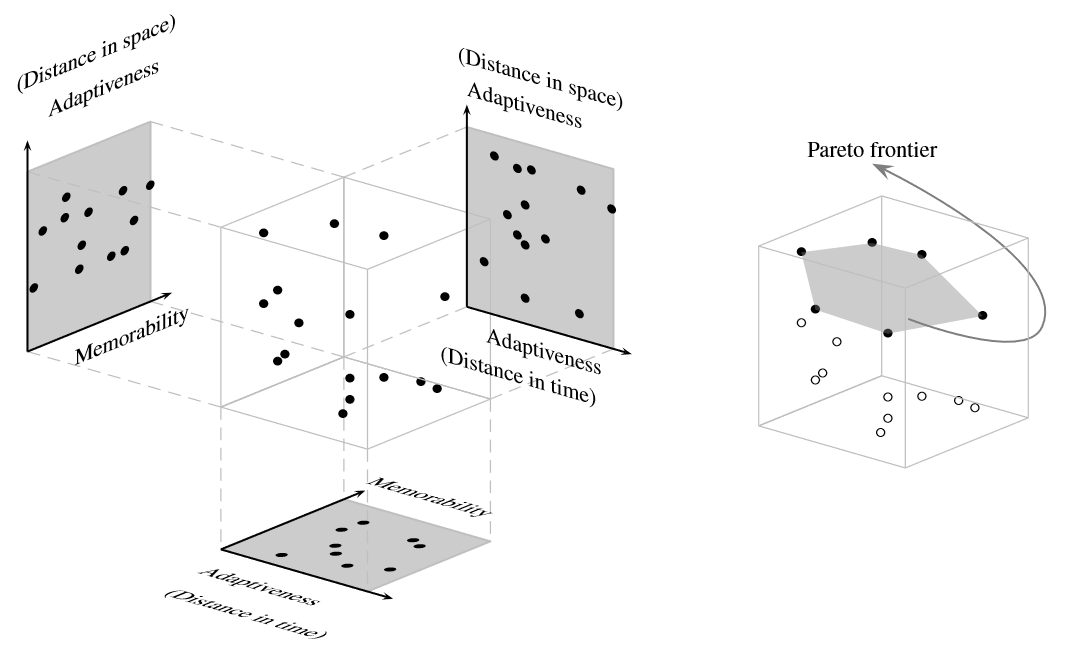
\includegraphics[height=2.30in]{pareto}
\end{figure}

\end{frame}

\section{Labeling Efforts}
\begin{frame}\frametitle{Research Questions}

\begin{enumerate}
\item Resources:
\begin{itemize}
\item How to build classification models fast?
\end{itemize}

\item Accuracy:
\begin{itemize}
\item How to deal with concept drifts?
\end{itemize}

\item Effort:
\begin{itemize}
\item \alert{How to reduce labeling effort?}
\end{itemize}

\end{enumerate}

\end{frame}

\section{Results}

\begin{frame}\frametitle{Evaluation}

\begin{itemize}
\item Measures used:
\begin{itemize}
\item Mean Squared Error.
\item RAM-Hours:
\begin{itemize}
\item A GB of RAM deployed for 1 hour execution.
\end{itemize}
\end{itemize}
\item Labeling Effort:
\begin{itemize}
\item Different batch sizes and $\delta$ values.
\end{itemize}
\item Three datasets:
\begin{itemize}
\item Brazilian elections 2010.
\item World Cup 2010.
\item Person of the Year 2010 (Assange vs. Zuckerberg)
\end{itemize}
\begin{itemize}
\item Baselines:
\begin{itemize}
\item AC $-$ Active Classifiers (KDD 2011)
\item HAT $-$ Hoeffding Adaptive Trees (JMLR 2011)
\item ILAC $-$ Incremental Lazy Classifiers (SIGIR 2011)
\end{itemize}
\end{itemize}
\end{itemize}

\end{frame}

\begin{frame}\frametitle{Evaluation}

\begin{itemize}
\item MSE and RAM-Hours
\end{itemize}

\begin{figure}
\centering
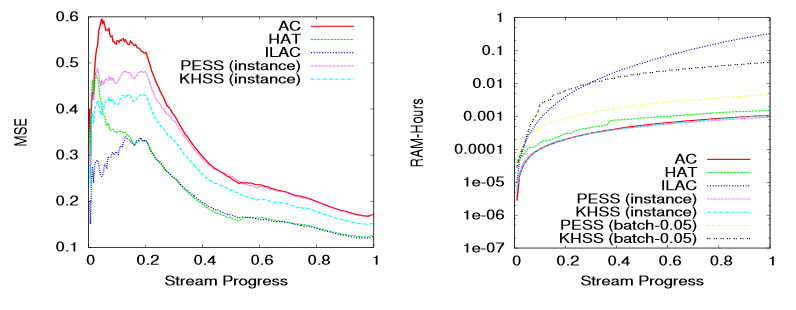
\includegraphics[height=1.70in]{results3}
\end{figure}

\end{frame}

\begin{frame}\frametitle{Evaluation}

\begin{itemize}
\item MSE and Labeling Effort
\end{itemize}

\begin{figure}
\centering
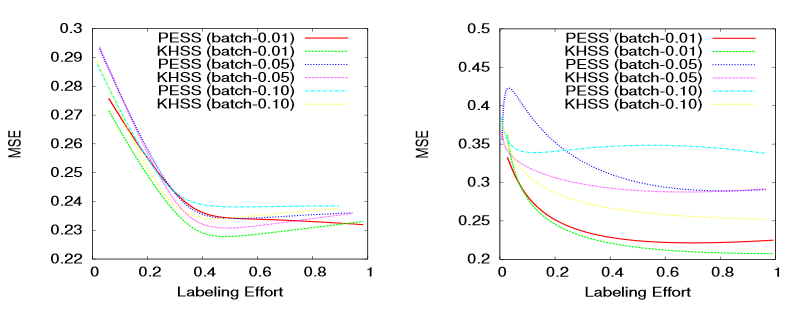
\includegraphics[height=1.70in]{results2}
\end{figure}

\end{frame}


\section{Conclusions}

\begin{frame}\frametitle{Conclusions}

\begin{itemize}
\item Sentiment analysis on Twitter streams.
\begin{itemize}
\item Limited computing and training resources.
\item Sentiment drifts.
\end{itemize}
\item Efficiency and accuracy.
\begin{itemize}
\item Incremental classifiers.
\item Pareto efficiency and compensation principle.
\end{itemize}
\item Our results.
\begin{itemize}
\item 50\% reduction in terms of labeling effort without impact on accuracy.
\end{itemize}
\item Future work includes:
\begin{itemize}
\item Other utility measures.
\item Other application scenarios.
\end{itemize}
\end{itemize}

\end{frame}






\section{Contact}
\begin{frame}{Thank you!}
\begin{center}
\tt adrianov@dcc.ufmg.br\\
\end{center}
\end{frame}

\end{document}


